\documentclass[tikz,border=15pt]{standalone}
\usepackage{amsmath,amssymb}
\usetikzlibrary{calc}

\begin{document}
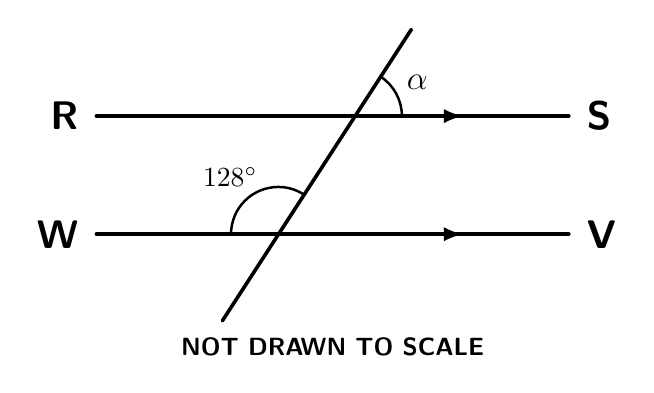
\begin{tikzpicture}[line cap=round, line join=round, scale=1.0]
  % Parallel lines RS and WV
  \coordinate (R_left) at (-0.5, 2.2);
  \coordinate (S_right) at (5.5, 2.2);
  \coordinate (W_left) at (-0.5, 0.7);
  \coordinate (V_right) at (5.5, 0.7);

  % Horizontal lines
  \draw[line width=1.3pt] (R_left) -- (S_right);
  \draw[line width=1.3pt] (W_left) -- (V_right);

  % Parallel indicator arrows
  \draw[line width=1.3pt, -{latex}] (3.8, 2.2) -- (4.15, 2.2);
  \draw[line width=1.3pt, -{latex}] (3.8, 0.7) -- (4.15, 0.7);

  % Transversal line
  \coordinate (T_bot) at (1.1, -0.4);
  \coordinate (T_top) at (3.5, 3.3);
  \draw[line width=1.3pt] (T_bot) -- (T_top);

  % Intersections
  \coordinate (Int_bot) at (1.81, 0.7);
  \coordinate (Int_top) at (2.78, 2.2);

  % Arcs & labels
  % 128 deg at bottom
  \draw[line width=0.9pt] ($(Int_bot) + (180:0.6)$) arc (180:57:0.6);
  \node[font=\normalsize] at ($(Int_bot) + (130:0.95)$) {$128^\circ$};

  % alpha at top
  \draw[line width=0.9pt] ($(Int_top) + (57:0.6)$) arc (57:0:0.6);
  \node[font=\large] at ($(Int_top) + (28:0.9)$) {$\alpha$};

  % Labels
  \node[left=3pt, font=\Large\sffamily\bfseries] at (R_left) {R};
  \node[right=3pt, font=\Large\sffamily\bfseries] at (S_right) {S};
  \node[left=3pt, font=\Large\sffamily\bfseries] at (W_left) {W};
  \node[right=3pt, font=\Large\sffamily\bfseries] at (V_right) {V};

  % Footer
  \node[below=14pt, font=\small\sffamily\bfseries] at (2.5, 0) {NOT DRAWN TO SCALE};

\end{tikzpicture}
\end{document}
